\documentclass[russian, 14pt]{beamer}
%\documentclass[handout]{beamer} %раздаточный материал
%\documentclass[aspectratio=169]{beamer}

%%% Работа с русским языком
\usepackage{cmap} %поиск в PDF
\usepackage{mathtext} %русские буквы в формулах
\usepackage[T2A]{fontenc} %кодировка
\usepackage[utf8]{inputenc} %кодировка исходного текста
\usepackage[english,russian]{babel} %локализация и переносы

%%Beamer по-русски
\newtheorem{rtheorem}{Теорема}
\newtheorem{rproof}{Доказательство}
\newtheorem{rexample}{Пример}

%%% Матпакеты
\usepackage{amsmath,amsfonts,amssymb,amsthm,mathtools} %AMS
\usepackage{icomma} %"Умная запятая": $0,2$ --  число, $0, 2$ -- перечисление

%% Номера формул
%\mathtoolsset{showonlyrefs=true} %Показывать номера только у тех в формул,
%на которые есть \eqref{} в тексте
%\usepackage{legno} %нумеризация формул слева

%%Свои команды
\DeclareMathOperator{\sgn}{\mathop{sgn}}

%%Перенос знаков в формулах (по Львовскому)
\newcommand*{\hm}[1]{#1\nobreak\discretionary{}
	{\hbox{$\mathsurround=0pt #1$}}{}}

%%%Работа с картинками
\usepackage{graphics} %Для вставки рисунков
\graphicspath{{images/}} %папки с картинками
\setlength\fboxsep{3pt} %отступ рамки \fbox{} от рисунка 
\setlength\fboxrule{1pt} %толщина линий рамки \fbox{}
\usepackage{wrapfig} %обтекание рисунков и таблиц текстом

%%%Работа с таблицами
\usepackage{array,tabularx,tabulary,booktabs} %дополнительная работа с таблицами
\usepackage{longtable} %длинные таблицы
\usepackage{multirow} %слияние строк в таблице

%%%Работа с видео и аудио
\usepackage{multimedia}
\usepackage{media9}
\usepackage{hyperref}

\usepackage{caption}

\usetheme{Rochester} %тема оформления
%beamer theme matrix
\usecolortheme{whale}

%%%Заголовок
\author[]{Панчишин Д.И.
\and Носков Р.И.
\and Пасютин А.С.
}
\title[Презентация]{Проект \textbf{«\LaTeX»}}
\subtitle{Выполнили студенты 1 курса, ФИТ-204:}
\date[]{}
\institute[]{\normalsize\textbf{КемГУ}}

\begin{document}
	
	\begin{frame}
		\maketitle
	\end{frame}

\begin{frame}
	\frametitle{Цели}
	\begin{itemize}
		\item Научиться делать документы с высококачественной версткой текста и формул
		\item Продемонстрировать группе возможности \LaTeX'а
	\end{itemize}
\end{frame}

\begin{frame}
	\frametitle{Задачи}
	\begin{itemize}
		\item Изучение инструментов и макропакетов \TeX’а
		\item Получение навыков верстки текста в \LaTeX'е
		\item Создание отчета по проекту в системе \LaTeX
	\end{itemize}
\end{frame}

\begin{frame}
	\frametitle{Индивидуальные задачи}
	\begin{enumerate}
		\item<1-> \textbf{Панчишин Даниил} - Тим-лид, создание тех задания, работа в \LaTeX’е с мат. формулами, рисунками и графиками;
		\item<2-> \textbf{Носков Роман} - Работа в \LaTeX’е с инструментами для верстки текста;
		\item<3-> \textbf{Пасютин Александр} - Работа в \LaTeX’е с инструментами для работы с презентациями.
	\end{enumerate}
\end{frame}

\begin{frame} \label{tab}
	\frametitle{Календарный план}
	\small{
	\begin{tabular}{|l|p{8,5cm}|}
		\hline
		18.02 & Распределение ролей, создание удаленного репозитория, составление календарного плана \\
		\hline
		4.03 & Изучение общего теоретического материала \\
		\hline
		18.03 & Начало работы над практической частью проекта \\
		\hline
		01.04 & Изучение отдельных аспектов \LaTeX’а, распределенных по ролям \\
		\hline
		15.04 & Создание презентации в \LaTeX, которая бы демонстрировала изученные навыки \\
		\hline
		29.04 & Создание отчета в \LaTeX, который бы демонстрировал изученные навыки
		\\
		\hline
		13.05 & Презентация результатов работы над проектом \\
		\hline
		27.05-31.05 & Защита проекта \\
		\hline
	\end{tabular}
	\hyperlink{button}{\beamerbutton{Вернуться обратно}}
}
\end{frame}

\begin{frame}
	\frametitle{Используемые средства}
\begin{figure}[h]
	\begin{center}
		\begin{minipage}[h]{0.4\linewidth}
			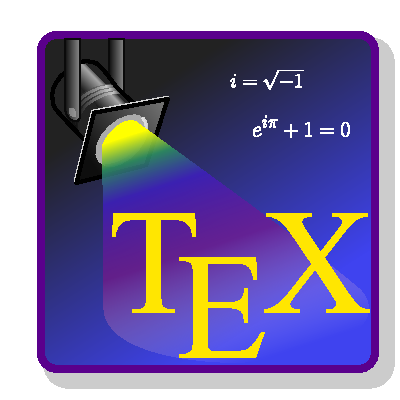
\includegraphics[width=5cm,height=5cm]{tex}
			\caption*{\huge{TeXStudio}}
		\end{minipage}
		\hfill											
		\begin{minipage}[h]{0.4\linewidth}
			
\includegraphics[width=5cm,height=5cm]{miktex}
			\caption*{\huge{MiKTeX}}
		\end{minipage}
	\end{center}
\end{figure}
\end{frame}

\begin{frame}
	\frametitle{Зачем использовать \TeX  для создания презентаций?}
	\begin{itemize}
		\item На слайдах отображаетя материал, набранный изначально в \LaTeX'е. 
		\item На слайдах много формул.
		\item Вам не хочется думать о переносимости файлов PowerPoint между различными версиями / компьютерами. Готовый файл pdf отображается везде. 
	\end{itemize}
\end{frame}

\begin{frame}
	\frametitle{Beamer}
	\begin{itemize}
		\item Beamer - класс для \LaTeX'а,специально предназначенный для создания презентаций.
		\item Позволяет настраивать внешний вид, переходы и т.п.
		\item Добавляет новые возможности к командам \TeX'а.
	\end{itemize}
\end{frame}

\begin{frame}
	\frametitle{Титульный слайд}
	\begin{block}{Преамбула}
		\textbackslash title[short title]\{long title\}
		
		
		\textbackslash subtitle[short subtitle]\{long subtitle\}
		
		
		\textbackslash author[short name]\{long name\}
		
		
		\textbackslash date[short date]\{long date\}
		
		
		\textbackslash institute[short name]\{long name\}
		
		
		\textbackslash titlepage
	\end{block}
\end{frame}

\begin{frame}
	\frametitle{Frame'ы}
	\begin{block}{Один кадр}
		\textbackslash begin\{frame\}
		
		
		\%код \LaTeX'а или текст 
		
		
		\textbackslash end\{frame\}
	\end{block}
\end{frame}

\begin{frame}
	\frametitle{Overlay'и}
		\begin{block}{Примеры overlay'ев}
			\pause \textbackslash pause
			
			
			\only<4-> {\textbackslash only<4->} 
			
			
			\uncover<3-> {\textbackslash uncover<3->}
			
			
			\alt<5> {\textbackslash alt<5>}{Сейчас не 5 кадр}
			
			
			\temporal<6>{Сейчас не 6 кадр}{\textbackslash temporal<6>}{6 кадр уже прошел}
			
			
			\begin{itemize}
				\item<7> {\textbackslash item<7>} 
			\end{itemize}
		\end{block}
\end{frame}

\begin{frame}
	\frametitle{Блоки}
	\begin{block}{Название блока}
		Содержимое блока
	\end{block}


	\textbackslash begin\{block\}\{Название блока\}
	
	
	Содержимое блока
	
	
	\textbackslash end\{block\}
\end{frame}

\begin{frame}
	\frametitle{Таблицы}
	\begin{flushleft}
	\textbackslash begin\{tabular\}\{|l|p{8,5cm}|\}
	
	
		\textbackslash hline
		
		
		18.02 \& Распределение ролей, создание удаленного репозитория, составление календарного плана \textbackslash\textbackslash
		
		
		\textbackslash hline


		...
		
		
		\textbackslash end\{tabular\}
		
		
		\hyperlink{tab}{\beamerbutton{Посмотреть таблицу}}
	\end{flushleft}
\end{frame}

\begin{frame} \label{button}
	\frametitle{Ссылки, кнопки, рисунки}
	\textbackslash hyperlink\{label\}\{\textbackslash beamerbutton\{Кнопка\}\}
	
	
	\textbackslash hyperlink\{label\}\{\textbackslash includegraphics[scale=0.3]\{kemsu\}\}
	
	
	\centering\hyperlink{video}{
\includegraphics[scale=0.3]{kemsu}}
\end{frame}

\begin{frame} \label{video}
	\frametitle{Видео}
	\includemedia[
	activate=pageopen,
	width=320pt,height=180pt,
	addresource=kem.mp4,
	flashvars={%
		source=kem.mp4
		&loop=true}
	]{}{VPlayer.swf}
\end{frame}

\begin{frame}
	\frametitle{Итоговый результат}
\end{frame}
\end{document}